\documentclass{standalone}
\usepackage{tikz}
\usetikzlibrary{patterns, positioning}

\begin{document}
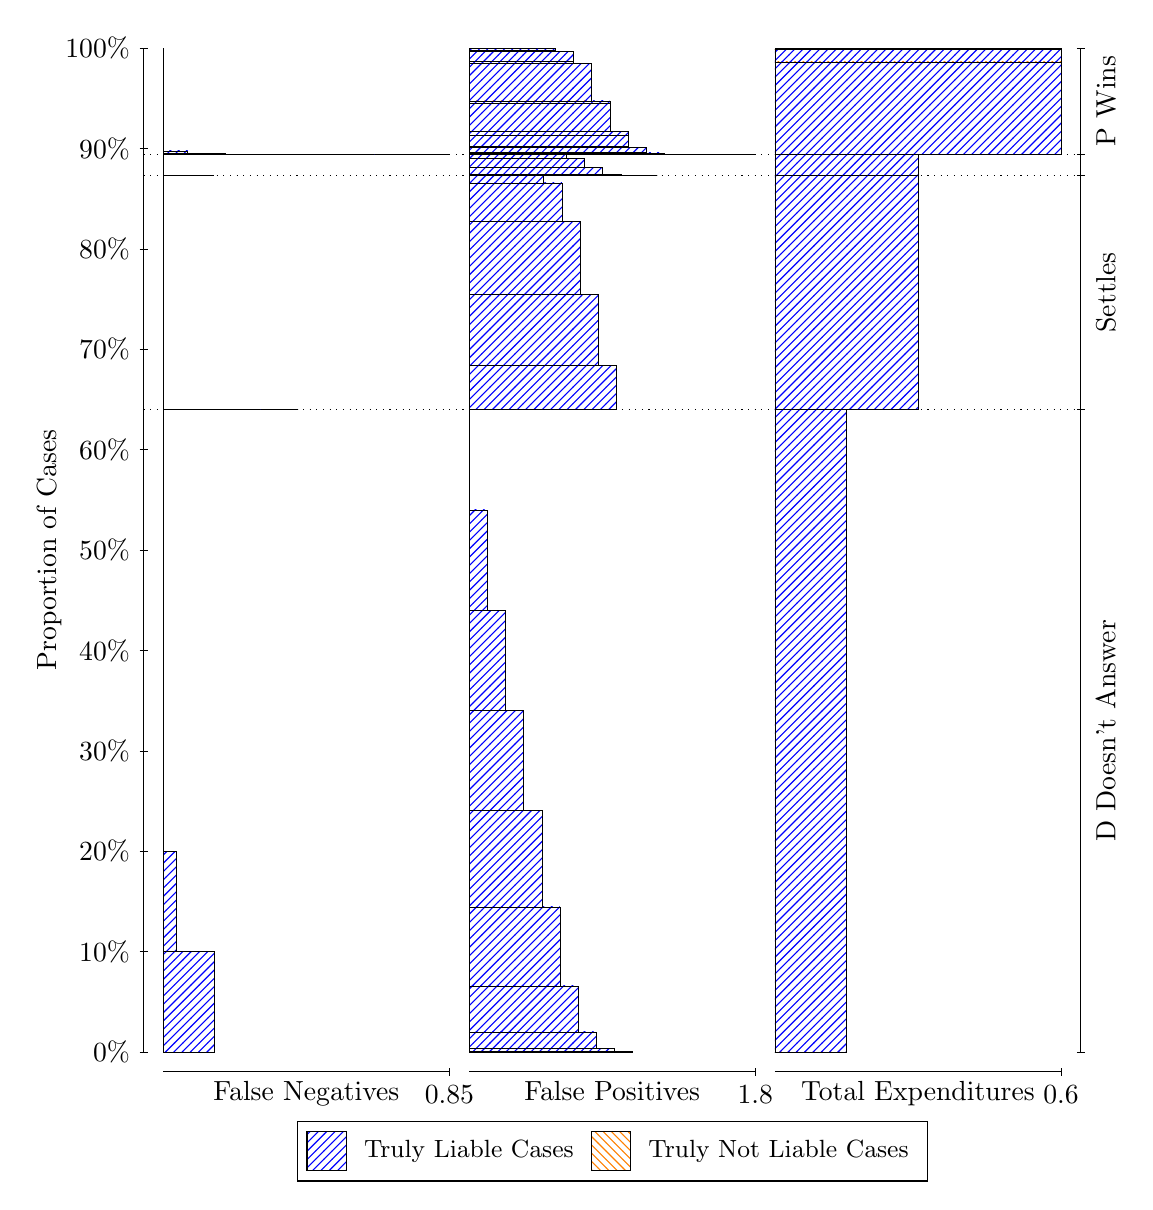
\begin{tikzpicture}
\draw[black, very thin] (1.5,1.75) -- (1.5,14.5);
\node[rotate=90, anchor=center] at (0.3, 8.125) {Proportion of Cases};
\draw[black, very thin] (1.45,1.75) -- (1.55,1.75);
\node[anchor=east] at (1.45, 1.75) {0\%};
\draw[black, very thin] (1.45,3.025) -- (1.55,3.025);
\node[anchor=east] at (1.45, 3.025) {10\%};
\draw[black, very thin] (1.45,4.3) -- (1.55,4.3);
\node[anchor=east] at (1.45, 4.3) {20\%};
\draw[black, very thin] (1.45,5.575) -- (1.55,5.575);
\node[anchor=east] at (1.45, 5.575) {30\%};
\draw[black, very thin] (1.45,6.85) -- (1.55,6.85);
\node[anchor=east] at (1.45, 6.85) {40\%};
\draw[black, very thin] (1.45,8.125) -- (1.55,8.125);
\node[anchor=east] at (1.45, 8.125) {50\%};
\draw[black, very thin] (1.45,9.4) -- (1.55,9.4);
\node[anchor=east] at (1.45, 9.4) {60\%};
\draw[black, very thin] (1.45,10.675) -- (1.55,10.675);
\node[anchor=east] at (1.45, 10.675) {70\%};
\draw[black, very thin] (1.45,11.95) -- (1.55,11.95);
\node[anchor=east] at (1.45, 11.95) {80\%};
\draw[black, very thin] (1.45,13.225) -- (1.55,13.225);
\node[anchor=east] at (1.45, 13.225) {90\%};
\draw[black, very thin] (1.45,14.5) -- (1.55,14.5);
\node[anchor=east] at (1.45, 14.5) {100\%};

\draw[black, very thin] (13.4,1.75) -- (13.4,14.5);
\draw[black, very thin] (13.35,1.75) -- (13.45,1.75);
\node[anchor=west] at (13.35, 1.75) {};
\draw[black, very thin] (13.35,9.909) -- (13.45,9.909);
\node[anchor=west] at (13.35, 9.909) {};
\draw[black, very thin] (13.35,12.885) -- (13.45,12.885);
\node[anchor=west] at (13.35, 12.885) {};
\draw[black, very thin] (13.35,13.15) -- (13.45,13.15);
\node[anchor=west] at (13.35, 13.15) {};
\draw[black, very thin] (13.35,14.5) -- (13.45,14.5);
\node[anchor=west] at (13.35, 14.5) {};

\draw[black, very thin, pattern color=blue, pattern=north east lines] (1.75,1.75) rectangle (2.3912,3.025);
\draw[black, very thin, pattern color=blue, pattern=north east lines] (1.75,3.025) rectangle (1.9162,4.3);
\draw[black, very thin, pattern color=orange, pattern=north west lines] (1.75,4.3) rectangle (1.75,4.3);
\draw[black, very thin, pattern color=blue, pattern=north east lines] (1.75,4.3) rectangle (1.75,9.909);
\draw[black, very thin, pattern color=blue, pattern=north east lines] (1.75,9.909) rectangle (3.4598,9.909);
\draw[black, very thin, pattern color=blue, pattern=north east lines] (1.75,9.909) rectangle (2.9849,9.909);
\draw[black, very thin, pattern color=blue, pattern=north east lines] (1.75,9.909) rectangle (2.5099,9.909);
\draw[black, very thin, pattern color=blue, pattern=north east lines] (1.75,9.909) rectangle (2.035,9.9091);
\draw[black, very thin, pattern color=orange, pattern=north west lines] (1.75,9.9091) rectangle (1.75,9.9091);
\draw[black, very thin, pattern color=blue, pattern=north east lines] (1.75,9.9091) rectangle (1.75,12.885);
\draw[black, very thin, pattern color=blue, pattern=north east lines] (1.75,12.885) rectangle (2.3912,12.885);
\draw[black, very thin, pattern color=blue, pattern=north east lines] (1.75,12.885) rectangle (1.9162,12.885);
\draw[black, very thin, pattern color=orange, pattern=north west lines] (1.75,12.885) rectangle (1.75,12.885);
\draw[black, very thin, pattern color=blue, pattern=north east lines] (1.75,12.885) rectangle (1.75,13.15);
\draw[black, very thin, pattern color=blue, pattern=north east lines] (1.75,13.15) rectangle (5.3833,13.15);
\draw[black, very thin, pattern color=blue, pattern=north east lines] (1.75,13.15) rectangle (4.9084,13.15);
\draw[black, very thin, pattern color=blue, pattern=north east lines] (1.75,13.15) rectangle (4.4334,13.15);
\draw[black, very thin, pattern color=blue, pattern=north east lines] (1.75,13.15) rectangle (3.9585,13.15);
\draw[black, very thin, pattern color=blue, pattern=north east lines] (1.75,13.15) rectangle (3.9585,13.15);
\draw[black, very thin, pattern color=blue, pattern=north east lines] (1.75,13.15) rectangle (3.4836,13.15);
\draw[black, very thin, pattern color=blue, pattern=north east lines] (1.75,13.15) rectangle (3.4836,13.15);
\draw[black, very thin, pattern color=blue, pattern=north east lines] (1.75,13.15) rectangle (3.4836,13.15);
\draw[black, very thin, pattern color=blue, pattern=north east lines] (1.75,13.15) rectangle (3.0086,13.15);
\draw[black, very thin, pattern color=blue, pattern=north east lines] (1.75,13.15) rectangle (3.0086,13.151);
\draw[black, very thin, pattern color=blue, pattern=north east lines] (1.75,13.151) rectangle (2.5337,13.151);
\draw[black, very thin, pattern color=blue, pattern=north east lines] (1.75,13.151) rectangle (2.5337,13.151);
\draw[black, very thin, pattern color=blue, pattern=north east lines] (1.75,13.151) rectangle (2.5337,13.158);
\draw[black, very thin, pattern color=blue, pattern=north east lines] (1.75,13.158) rectangle (2.0587,13.159);
\draw[black, very thin, pattern color=blue, pattern=north east lines] (1.75,13.159) rectangle (2.0587,13.193);
\draw[black, very thin, pattern color=blue, pattern=north east lines] (1.75,13.193) rectangle (2.0587,13.193);
\draw[black, very thin, pattern color=orange, pattern=north west lines] (1.75,13.193) rectangle (1.75,13.193);
\draw[black, very thin, pattern color=blue, pattern=north east lines] (1.75,13.193) rectangle (1.75,14.5);
\draw[black, very thin, pattern color=orange, pattern=north west lines] (5.6333,1.75) rectangle (7.7095,1.75);
\draw[black, very thin, pattern color=blue, pattern=north east lines] (5.6333,1.75) rectangle (7.7095,1.7548);
\draw[black, very thin, pattern color=blue, pattern=north east lines] (5.6333,1.7548) rectangle (7.4788,1.796);
\draw[black, very thin, pattern color=blue, pattern=north east lines] (5.6333,1.796) rectangle (7.2481,2.0041);
\draw[black, very thin, pattern color=blue, pattern=north east lines] (5.6333,2.0041) rectangle (7.0175,2.5904);
\draw[black, very thin, pattern color=blue, pattern=north east lines] (5.6333,2.5904) rectangle (6.7868,3.5938);
\draw[black, very thin, pattern color=blue, pattern=north east lines] (5.6333,3.5938) rectangle (6.5561,4.8141);
\draw[black, very thin, pattern color=blue, pattern=north east lines] (5.6333,4.8141) rectangle (6.3254,6.0842);
\draw[black, very thin, pattern color=blue, pattern=north east lines] (5.6333,6.0842) rectangle (6.0947,7.359);
\draw[black, very thin, pattern color=blue, pattern=north east lines] (5.6333,7.359) rectangle (5.864,8.634);
\draw[black, very thin, pattern color=blue, pattern=north east lines] (5.6333,8.634) rectangle (5.6333,9.909);
\draw[black, very thin, pattern color=orange, pattern=north west lines] (5.6333,9.909) rectangle (7.5019,9.909);
\draw[black, very thin, pattern color=blue, pattern=north east lines] (5.6333,9.909) rectangle (7.5019,10.473);
\draw[black, very thin, pattern color=blue, pattern=north east lines] (5.6333,10.473) rectangle (7.2712,11.371);
\draw[black, very thin, pattern color=blue, pattern=north east lines] (5.6333,11.371) rectangle (7.0405,12.299);
\draw[black, very thin, pattern color=blue, pattern=north east lines] (5.6333,12.299) rectangle (6.8098,12.786);
\draw[black, very thin, pattern color=blue, pattern=north east lines] (5.6333,12.786) rectangle (6.5792,12.88);
\draw[black, very thin, pattern color=blue, pattern=north east lines] (5.6333,12.88) rectangle (6.3485,12.885);
\draw[black, very thin, pattern color=blue, pattern=north east lines] (5.6333,12.885) rectangle (6.1178,12.885);
\draw[black, very thin, pattern color=blue, pattern=north east lines] (5.6333,12.885) rectangle (5.8871,12.885);
\draw[black, very thin, pattern color=blue, pattern=north east lines] (5.6333,12.885) rectangle (5.6564,12.885);
\draw[black, very thin, pattern color=blue, pattern=north east lines] (5.6333,12.885) rectangle (5.6333,12.885);
\draw[black, very thin, pattern color=orange, pattern=north west lines] (5.6333,12.885) rectangle (8.021,12.885);
\draw[black, very thin, pattern color=blue, pattern=north east lines] (5.6333,12.885) rectangle (8.021,12.885);
\draw[black, very thin, pattern color=blue, pattern=north east lines] (5.6333,12.885) rectangle (7.7903,12.885);
\draw[black, very thin, pattern color=blue, pattern=north east lines] (5.6333,12.885) rectangle (7.5596,12.897);
\draw[black, very thin, pattern color=blue, pattern=north east lines] (5.6333,12.897) rectangle (7.3289,12.981);
\draw[black, very thin, pattern color=blue, pattern=north east lines] (5.6333,12.981) rectangle (7.0982,13.103);
\draw[black, very thin, pattern color=blue, pattern=north east lines] (5.6333,13.103) rectangle (6.8675,13.146);
\draw[black, very thin, pattern color=blue, pattern=north east lines] (5.6333,13.146) rectangle (6.6368,13.15);
\draw[black, very thin, pattern color=blue, pattern=north east lines] (5.6333,13.15) rectangle (6.4061,13.15);
\draw[black, very thin, pattern color=blue, pattern=north east lines] (5.6333,13.15) rectangle (6.1754,13.15);
\draw[black, very thin, pattern color=blue, pattern=north east lines] (5.6333,13.15) rectangle (5.9448,13.15);
\draw[black, very thin, pattern color=orange, pattern=north west lines] (5.6333,13.15) rectangle (9.2667,13.15);
\draw[black, very thin, pattern color=blue, pattern=north east lines] (5.6333,13.15) rectangle (9.2667,13.15);
\draw[black, very thin, pattern color=orange, pattern=north west lines] (5.6333,13.15) rectangle (9.036,13.15);
\draw[black, very thin, pattern color=blue, pattern=north east lines] (5.6333,13.15) rectangle (9.036,13.15);
\draw[black, very thin, pattern color=orange, pattern=north west lines] (5.6333,13.15) rectangle (8.8053,13.15);
\draw[black, very thin, pattern color=blue, pattern=north east lines] (5.6333,13.15) rectangle (8.8053,13.15);
\draw[black, very thin, pattern color=blue, pattern=north east lines] (5.6333,13.15) rectangle (8.5746,13.15);
\draw[black, very thin, pattern color=orange, pattern=north west lines] (5.6333,13.15) rectangle (8.5746,13.15);
\draw[black, very thin, pattern color=blue, pattern=north east lines] (5.6333,13.15) rectangle (8.5746,13.151);
\draw[black, very thin, pattern color=orange, pattern=north west lines] (5.6333,13.151) rectangle (8.3439,13.151);
\draw[black, very thin, pattern color=blue, pattern=north east lines] (5.6333,13.151) rectangle (8.3439,13.152);
\draw[black, very thin, pattern color=blue, pattern=north east lines] (5.6333,13.152) rectangle (8.3439,13.153);
\draw[black, very thin, pattern color=orange, pattern=north west lines] (5.6333,13.153) rectangle (8.1132,13.153);
\draw[black, very thin, pattern color=blue, pattern=north east lines] (5.6333,13.153) rectangle (8.1132,13.167);
\draw[black, very thin, pattern color=blue, pattern=north east lines] (5.6333,13.167) rectangle (8.1132,13.168);
\draw[black, very thin, pattern color=blue, pattern=north east lines] (5.6333,13.168) rectangle (7.8825,13.173);
\draw[black, very thin, pattern color=orange, pattern=north west lines] (5.6333,13.173) rectangle (7.8825,13.173);
\draw[black, very thin, pattern color=blue, pattern=north east lines] (5.6333,13.173) rectangle (7.8825,13.238);
\draw[black, very thin, pattern color=blue, pattern=north east lines] (5.6333,13.238) rectangle (7.6519,13.251);
\draw[black, very thin, pattern color=orange, pattern=north west lines] (5.6333,13.251) rectangle (7.6519,13.251);
\draw[black, very thin, pattern color=blue, pattern=north east lines] (5.6333,13.251) rectangle (7.6519,13.39);
\draw[black, very thin, pattern color=blue, pattern=north east lines] (5.6333,13.39) rectangle (7.6519,13.441);
\draw[black, very thin, pattern color=orange, pattern=north west lines] (5.6333,13.441) rectangle (7.4212,13.441);
\draw[black, very thin, pattern color=blue, pattern=north east lines] (5.6333,13.441) rectangle (7.4212,13.798);
\draw[black, very thin, pattern color=blue, pattern=north east lines] (5.6333,13.798) rectangle (7.4212,13.827);
\draw[black, very thin, pattern color=blue, pattern=north east lines] (5.6333,13.827) rectangle (7.4212,13.828);
\draw[black, very thin, pattern color=orange, pattern=north west lines] (5.6333,13.828) rectangle (7.1905,13.828);
\draw[black, very thin, pattern color=blue, pattern=north east lines] (5.6333,13.828) rectangle (7.1905,14.307);
\draw[black, very thin, pattern color=blue, pattern=north east lines] (5.6333,14.307) rectangle (7.1905,14.307);
\draw[black, very thin, pattern color=blue, pattern=north east lines] (5.6333,14.307) rectangle (6.9598,14.335);
\draw[black, very thin, pattern color=blue, pattern=north east lines] (5.6333,14.335) rectangle (6.9598,14.458);
\draw[black, very thin, pattern color=blue, pattern=north east lines] (5.6333,14.458) rectangle (6.9598,14.458);
\draw[black, very thin, pattern color=blue, pattern=north east lines] (5.6333,14.458) rectangle (6.7291,14.471);
\draw[black, very thin, pattern color=blue, pattern=north east lines] (5.6333,14.471) rectangle (6.7291,14.492);
\draw[black, very thin, pattern color=blue, pattern=north east lines] (5.6333,14.492) rectangle (6.7291,14.493);
\draw[black, very thin, pattern color=blue, pattern=north east lines] (5.6333,14.493) rectangle (6.4984,14.495);
\draw[black, very thin, pattern color=blue, pattern=north east lines] (5.6333,14.495) rectangle (6.4984,14.499);
\draw[black, very thin, pattern color=blue, pattern=north east lines] (5.6333,14.499) rectangle (6.4984,14.499);
\draw[black, very thin, pattern color=blue, pattern=north east lines] (5.6333,14.499) rectangle (6.4984,14.499);
\draw[black, very thin, pattern color=blue, pattern=north east lines] (5.6333,14.499) rectangle (6.2677,14.5);
\draw[black, very thin, pattern color=blue, pattern=north east lines] (5.6333,14.5) rectangle (6.2677,14.5);
\draw[black, very thin, pattern color=blue, pattern=north east lines] (5.6333,14.5) rectangle (6.037,14.5);
\draw[black, very thin, pattern color=blue, pattern=north east lines] (5.6333,14.5) rectangle (6.037,14.5);
\draw[black, very thin, pattern color=blue, pattern=north east lines] (5.6333,14.5) rectangle (5.8063,14.5);
\draw[black, very thin, pattern color=blue, pattern=north east lines] (5.6333,14.5) rectangle (5.8063,14.5);
\draw[black, very thin, pattern color=blue, pattern=north east lines] (5.6333,14.5) rectangle (5.6333,14.5);
\draw[black, very thin, pattern color=orange, pattern=north west lines] (9.5167,1.75) rectangle (10.425,1.75);
\draw[black, very thin, pattern color=blue, pattern=north east lines] (9.5167,1.75) rectangle (10.425,9.909);
\draw[black, very thin, pattern color=orange, pattern=north west lines] (9.5167,9.909) rectangle (11.333,9.909);
\draw[black, very thin, pattern color=blue, pattern=north east lines] (9.5167,9.909) rectangle (11.333,12.885);
\draw[black, very thin, pattern color=orange, pattern=north west lines] (9.5167,12.885) rectangle (11.333,12.885);
\draw[black, very thin, pattern color=blue, pattern=north east lines] (9.5167,12.885) rectangle (11.333,13.15);
\draw[black, very thin, pattern color=orange, pattern=north west lines] (9.5167,13.15) rectangle (13.15,13.15);
\draw[black, very thin, pattern color=blue, pattern=north east lines] (9.5167,13.15) rectangle (13.15,14.323);
\draw[black, very thin, pattern color=orange, pattern=north west lines] (9.5167,14.323) rectangle (13.15,14.323);
\draw[black, very thin, pattern color=blue, pattern=north east lines] (9.5167,14.323) rectangle (13.15,14.482);
\draw[black, very thin, pattern color=orange, pattern=north west lines] (9.5167,14.482) rectangle (13.15,14.482);
\draw[black, very thin, pattern color=blue, pattern=north east lines] (9.5167,14.482) rectangle (13.15,14.5);
\draw[black, dotted] (1.5,9.909) -- (13.4,9.909);
\draw[black, dotted] (1.5,12.885) -- (13.4,12.885);
\draw[black, dotted] (1.5,13.15) -- (13.4,13.15);
\draw[black, very thin] (1.75,1.5) -- (5.3833,1.5);
\node[anchor=north] at (3.5667, 1.5) {False Negatives};
\draw[black, very thin] (5.3833,1.45) -- (5.3833,1.55);
\node[anchor=north] at (5.3833, 1.45) {0.85};

\draw[black, very thin] (5.6333,1.5) -- (9.2667,1.5);
\node[anchor=north] at (7.45, 1.5) {False Positives};
\draw[black, very thin] (9.2667,1.45) -- (9.2667,1.55);
\node[anchor=north] at (9.2667, 1.45) {1.8};

\draw[black, very thin] (9.5167,1.5) -- (13.15,1.5);
\node[anchor=north] at (11.333, 1.5) {Total Expenditures};
\draw[black, very thin] (13.15,1.45) -- (13.15,1.55);
\node[anchor=north] at (13.15, 1.45) {0.6};

\node[black, centered, rotate=90] at (13.72, 5.8295) {D Doesn't Answer};
\node[black, centered, rotate=90] at (13.72, 11.397) {Settles};

\node[black, centered, rotate=90] at (13.72, 13.825) {P Wins};

\draw (7.449999999999999,1.5) node[draw=none] (baseCoordinate) {};
\begin{scope}[align=center]
        \matrix[scale=0.5, draw=black, below=0.5cm of baseCoordinate, nodes={draw}, column sep=0.1cm]{
            \node[rectangle, draw, minimum width=0.5cm, minimum height=0.5cm, pattern=north east lines, pattern color=blue] {}; &
            \node[draw=none, font=\small] (B) {Truly Liable Cases}; &
            \node[rectangle, draw, minimum width=0.5cm, minimum height=0.5cm, pattern=north west lines, pattern color=orange] {}; &
            \node[draw=none, font=\small] (B) {Truly Not Liable Cases}; \\
            };
\end{scope}

\end{tikzpicture}
\end{document}